\documentclass[10.5pt,a4paper]{article}
\usepackage[a4paper,margin=2.2cm,top=2.3cm,bottom=2.4cm]{geometry}
\usepackage{fontspec}
\usepackage{unicode-math}
\setmainfont{TeX Gyre Pagella}
\setsansfont{Inter}[Scale=0.88]
\setmonofont{DejaVu Sans Mono}[Scale=0.80]
\setmathfont{DejaVu Math TeX Gyre}[Scale=0.95]
\usepackage{microtype}
\usepackage{xcolor}
\definecolor{accent}{HTML}{1F4E79}
\definecolor{muted}{HTML}{5F6670}
\definecolor{codebg}{HTML}{F6F7F9}
\definecolor{rule}{HTML}{D9DCE1}
\usepackage{graphicx}
\usepackage{booktabs,tabularx,array}
\usepackage{enumitem}
\setlist{nosep,leftmargin=1.4em,topsep=3pt}
\usepackage[font=small,labelfont={bf,sf},labelsep=period,skip=4pt]{caption}
\usepackage{titlesec}
\titleformat{\section}{\sffamily\large\bfseries\color{accent}}{\thesection}{0.7em}{}
\titleformat{\subsection}{\sffamily\normalsize\bfseries}{\thesubsection}{0.6em}{}
\titleformat{\subsubsection}[runin]{\sffamily\small\bfseries}{}{0em}{}[.]
\titlespacing*{\section}{0pt}{14pt}{6pt}
\titlespacing*{\subsection}{0pt}{10pt}{4pt}
\usepackage{fancyhdr}
\pagestyle{fancy}\fancyhf{}
\renewcommand{\headrulewidth}{0.4pt}
\renewcommand{\headrule}{\hbox to\headwidth{\color{rule}\leaders\hrule height \headrulewidth\hfill}}
\fancyhead[L]{\sffamily\footnotesize\color{muted}\ReportShortTitle}
\fancyhead[R]{\sffamily\footnotesize\color{muted}S. K. Eshraghi Naeini}
\fancyfoot[C]{\sffamily\footnotesize\color{muted}\thepage}
\usepackage{listings}
\lstdefinelanguage{VerilogX}[]{Verilog}{morekeywords={localparam,integer,genvar,generate,endgenerate}}
\lstset{language=VerilogX,basicstyle=\ttfamily\footnotesize,keywordstyle=\color{accent}\bfseries,
  commentstyle=\color{muted}\itshape,stringstyle=\color{teal!70!black},numbers=left,numberstyle=\tiny\color{muted},
  numbersep=6pt,backgroundcolor=\color{codebg},frame=single,rulecolor=\color{rule},framesep=4pt,
  xleftmargin=14pt,breaklines=true,columns=fullflexible,keepspaces=true,showstringspaces=false,
  tabsize=4,aboveskip=6pt,belowskip=6pt}
\usepackage{tikz}
\usetikzlibrary{arrows.meta,positioning,shapes.geometric,calc,fit,automata}
\tikzset{blk/.style={draw=accent,thick,fill=accent!6,rounded corners=2pt,minimum height=8mm,minimum width=20mm,align=center,font=\sffamily\small},
         io/.style={font=\sffamily\footnotesize,align=center},
         arr/.style={-{Stealth[length=2mm]},semithick},
         st/.style={state,draw=accent,thick,fill=accent!6,minimum size=9mm,font=\sffamily\footnotesize,inner sep=1pt,align=center}}
\usepackage{xurl}
\usepackage[colorlinks=true,linkcolor=accent,urlcolor=accent,citecolor=accent]{hyperref}
\usepackage{siunitx}
\sisetup{group-separator={,},group-minimum-digits=4}
\newcommand{\sig}[1]{\texttt{#1}}
\newcommand{\pass}{\textcolor{green!45!black}{\textsf{\textbf{PASS}}}}
\newcommand{\repo}{https://github.com/seyedkiarash/seyedkiarash.github.io/tree/main/labs/logic-circuits-lab}
\newcommand{\note}[1]{\par\smallskip\noindent\colorbox{accent!7}{\parbox{\dimexpr\linewidth-2\fboxsep}{\small #1}}\par\smallskip}
\setlength{\parindent}{0pt}
\setlength{\parskip}{4pt}

\newcommand{\ReportTitle}[3]{%
  \thispagestyle{plain}
  {\sffamily\small\color{muted}Logic Circuits Laboratory \textbullet\ Department of Electrical Engineering, Sharif University of Technology\par}
  \vspace{2pt}
  {\sffamily\LARGE\bfseries #1\par}
  \vspace{1pt}
  {\sffamily\Large #2\par}
  \vspace{6pt}
  {\color{rule}\hrule height 0.6pt}
  \vspace{5pt}
  {\small
  \begin{tabular}{@{}l@{\hspace{2em}}l@{}}
    \textcolor{muted}{Student}  & Seyed Kiarash Eshraghi Naeini (403101383)\\
    \textcolor{muted}{Instructor} & Dr.\ Mohammad Reza Movahhedin \quad\textcolor{muted}{Teaching assistant:} Hossein Moghim\\
    \textcolor{muted}{Semester} & Fall 2025 \quad\textcolor{muted}{session:} #3\\
    \textcolor{muted}{Platform} & Zynq-7010 (XC7Z010-CLG400-1), \SI{50}{MHz} clock, Vivado 2019.1
  \end{tabular}\par}
  \vspace{4pt}
  {\color{rule}\hrule height 0.6pt}
  \vspace{8pt}}

\newcommand{\ReportShortTitle}{Experiment 4 -- Adders, overflow and Hamming codes}
\begin{document}
\ReportTitle{Experiment 4}{Adders, Two's-Complement Overflow and Hamming Error-Correcting Codes}{16--17 November 2025}

\section*{Summary}
The first part of this experiment builds arithmetic from the bottom up: a seven-segment decoder, a
3-bit ripple-carry adder made of full adders (themselves made of half adders), and a 4-bit two's-complement
adder/subtractor with overflow detection and a sign-magnitude display. The second part implements the
Hamming(7,4) single-error-correcting code: encoder, decoder, a noisy ``transmission line'' controlled from
the switches and buttons, and finally the extended (8,4) SECDED code that also detects double errors.
All seven designs were verified exhaustively for this report (7/7 pass), including every single- and
double-error pattern for every data word. Code: \url{\repo/lab04-adders-hamming}.

\section{Part 1 -- Hexadecimal display}
\sig{Hex\_to\_7\_seg} decodes \sig{DIP[3:0]} into the segment pattern of \texttt{0}--\texttt{F}; the segments
of the extension board are active-low, so the positive-logic patterns are inverted. The module was also
packaged as an IP and instantiated in an IP-Integrator block design. Test: 256 DIP settings, 0 errors.

\section{Part 2 -- 3-bit ripple-carry adder}
A half adder gives $s=a\oplus b$, $c=ab$; two half adders and an OR gate form a full adder with
$c_\text{out}=ab+c_\text{in}(a\oplus b)$; three full adders chained through their carries form the 3-bit
adder. With $A=\sig{DIP[3:1]}$, $B=\sig{DIP[6:4]}$ and $c_\text{in}=\sig{DIP[7]}$, the 4-bit result
$\{c_\text{out},S\}$ (0--15) is shown in hexadecimal. Test: all 256 combinations, 0 errors.

\section{Part 3 -- Adder/subtractor with overflow}
\subsection{Design}
For subtraction, $A-B=A+\overline{B}+1$: every bit of $B$ passes through an XOR with the operation
signal \sig{Op}, which is also the carry-in of the first stage. With 4-bit two's-complement operands
(-8\ldots7) the result overflows when the carry \emph{into} the sign bit differs from the carry
\emph{out of} it, $V=c_3\oplus c_4$. The result is converted to sign and magnitude for display: the
magnitude appears on the seven-segment digit, \sig{LED[9]} shows a minus sign and \sig{LED[0]} signals
overflow -- in which case the digit is switched off (Fig.~\ref{fig:addsub}).
\begin{figure}[h]
\centering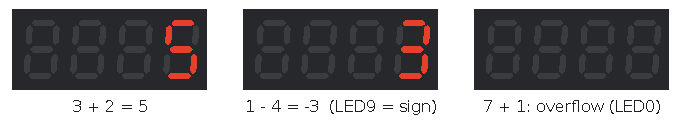
\includegraphics[width=0.62\linewidth]{figures/lab04_part3.pdf}
\caption{Part 3 display for a positive result, a negative result and an overflow.}\label{fig:addsub}
\end{figure}

\subsection{Verification}
All $256\times2$ operand/operation combinations were compared with integer arithmetic: the 128 results
outside $-8\ldots7$ are flagged as overflow with the digit blanked, and all 384 others show the correct
magnitude and sign. 0 errors.

\section{Parts 4--5 -- Hamming(7,4) encoder and decoder}
\subsection{Code construction}
The four data bits $x_0\ldots x_3$ and three parity bits $p_0,p_1,p_2$ occupy the positions 1--7 of the
code word so that each parity bit sits at a power-of-two position and covers the positions whose index
has the corresponding bit set (Table~\ref{tab:ham}). With even parity
\[
p_0=x_0\oplus x_1\oplus x_3,\qquad p_1=x_0\oplus x_2\oplus x_3,\qquad p_2=x_1\oplus x_2\oplus x_3 .
\]
\begin{table}[h]
\centering\small
\caption{Hamming(7,4) layout; \textbullet\ marks the positions checked by each parity bit.}\label{tab:ham}
\begin{tabular}{@{}lccccccc@{}}
\toprule
Position & 1 & 2 & 3 & 4 & 5 & 6 & 7\\
Bit & $p_0$ & $p_1$ & $x_0$ & $p_2$ & $x_1$ & $x_2$ & $x_3$\\
\midrule
$p_0$ (bit 0 of position) & \textbullet & & \textbullet & & \textbullet & & \textbullet\\
$p_1$ (bit 1) & & \textbullet & \textbullet & & & \textbullet & \textbullet\\
$p_2$ (bit 2) & & & & \textbullet & \textbullet & \textbullet & \textbullet\\
\bottomrule
\end{tabular}
\end{table}

\subsection{Decoding}
The decoder recomputes the three checks, $c_0=p_0\oplus x_0\oplus x_1\oplus x_3$ and so on. Because each
position is covered by exactly the checks named by its binary index, the syndrome $\{c_2,c_1,c_0\}$
\emph{is} the position of a single flipped bit (0: no error). Data bits at positions 3, 5, 6 and 7 are
inverted when the syndrome points at them; the syndrome is shown on the seven-segment display.

\subsection{Verification}
Encoder: for all 16 data words the three parity checks of the code word are even and the data bits are
in place. Decoder: every data word with no error and with each of the 7 single-bit errors
(128 cases) -- the data is recovered and the displayed position equals the flipped position.

\section{Part 6 -- Encoder, noisy channel and decoder}
The encoder output passes through a ``transmission line'' that XORs it with a 7-bit noise vector set by
\sig{DIP[7:5]} and the four (active-low) buttons; the decoder output is shown on \sig{LED[4:1]}.
Every data word was tested with every noise pattern of weight 0, 1 and 2:
\begin{itemize}
  \item all \textbf{128} cases with no or one error are corrected;
  \item all \textbf{336} double-error cases are decoded \emph{wrongly}. This is the expected limitation of a
        distance-3 code: two errors produce a non-zero syndrome that points at a third, correct bit, so the
        decoder ``corrects'' it and outputs a wrong word without any warning.
\end{itemize}

\section{Part 7 -- Extended Hamming (8,4) SECDED}
An eighth bit, the parity of the whole 7-bit code word, raises the minimum distance to 4. The decoder
combines the syndrome $s$ with the overall parity check $P$:
\begin{table}[h]
\centering\small
\begin{tabular}{@{}llll@{}}
\toprule
$s$ & $P$ & Interpretation & Output\\
\midrule
0 & even & no error & data, display \texttt{0}\\
$\neq0$ & odd & single error at position $s$ & corrected data, display $s$\\
0 & odd & the overall parity bit flipped & data, display \texttt{0}\\
$\neq0$ & even & \textbf{double error} -- detected, not correctable & \texttt{EE} on two digits, \sig{LED[4:1]} = \texttt{1111}\\
\bottomrule
\end{tabular}
\end{table}
\begin{figure}[h]
\centering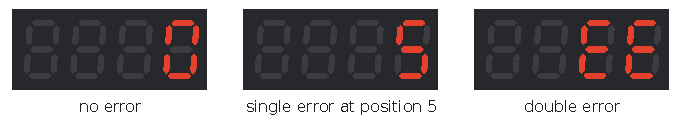
\includegraphics[width=0.62\linewidth]{figures/lab04_part7.pdf}
\caption{Part 7 display: no error, a corrected single error and a detected double error.}
\end{figure}

Verification over all data words and all noise patterns of weight $\leq2$ on the 8-bit word: the
\textbf{144} cases with no or one error are corrected and all \textbf{448} double-error cases are
detected. Compared with Part 6, the extra parity bit turns 336 silent miscorrections into 448 reported
errors.

\section{Implementation results}
All designs of this experiment are purely combinational (no flip-flops, no clock constraint). The
SECDED design of Part 7 uses \textbf{17 LUTs} in the Vivado implementation of the lab session (33 I/O
pins); Yosys synthesis of the other parts gives 3--20 LUTs each.

\section{Verification summary}
\begin{table}[h]
\centering\small
\begin{tabularx}{\linewidth}{@{}lXr@{}}
\toprule
Testbench & What is checked (exhaustive) & Result\\
\midrule
\sig{tb\_part1} & 256 DIP settings against a reference decoder & \pass\\
\sig{tb\_part2} & all 256 $(A,B,c_\text{in})$ combinations & \pass\\
\sig{tb\_part3} & 512 cases, overflow, sign and magnitude & \pass\\
\sig{tb\_part4} & 16 code words: parity checks and data positions & \pass\\
\sig{tb\_part5} & 16 words $\times$ (no error + 7 single errors) & \pass\\
\sig{tb\_part6} & 16 words $\times$ all noise patterns of weight $\leq2$ & \pass\\
\sig{tb\_part7} & 16 words $\times$ all 8-bit noise patterns of weight $\leq2$ & \pass\\
\bottomrule
\end{tabularx}
\end{table}
No functional changes were needed in this experiment; the cleaned code shares the half/full-adder cells
between the parts and has English comments.

\section{Conclusion}
Hierarchical design -- half adder, full adder, ripple-carry adder, adder/subtractor -- keeps each
module trivial while the whole performs signed arithmetic with correct overflow detection. The Hamming
experiments show both sides of a distance-3 code: every single error is corrected, but double errors are
silently miscorrected; one extra parity bit (SECDED) converts all of those into detected errors.

\end{document}
